\documentclass[../../spr.tex]{subfiles}

\begin{document}


\section{Implementacja}

\subsection{Opis głównych funkcjonalności aplikacji}

Aplikacja do zarządzania siłownią została zaprojektowana z myślą o różnych rolach użytkowników: klientach, pracownikach, trenerach oraz menadżerach. W zależności od przypisanej roli dostępne są różne funkcjonalności.

\begin{itemize}
  \item \textbf{Klient} może:
  \begin{itemize}
    \item Przeglądać status swojego karnetu.
    \item Śledzić swój postęp treningowy.
    \item Przeglądać i zapisywać się na dostępne sesje treningowe.
    \item Przeglądać historię treningów.
  \end{itemize}

  \item \textbf{Menadżer} ma możliwość:
  \begin{itemize}
    \item Tworzenia nowych pracowników poprzez formularz.
    \item Przeglądania listy klientów i pracowników.
    \item Zarządzania salami treningowymi oraz zadaniami serwisowymi.
  \end{itemize}
    \item \textbf{Pracownik} ma możliwość:
  \begin{itemize}
    \item Przeglądania listy klientów.
    \item Sprawdzania ważności karnetów.
    \item Zgłaszania usterek i tworzenia zadań serwisowych.
  \end{itemize}

  \item \textbf{Trener} może:
  \begin{itemize}
    \item Przeglądać przypisanych podopiecznych.
    \item Tworzyć i edytować plany treningowe.
    \item Zarządzać kalendarzem sesji treningowych.
  \end{itemize}

\end{itemize}

Aplikacja obsługuje różne widoki dla użytkowników w zależności od ich roli i zapewnia prosty oraz intuicyjny interfejs użytkownika, co przedstawiono na poniższych zrzutach ekranu.

\vspace{8pt}

\noindent\textit{Ze względu na dużą ilość zakładek pokazane zostały najczęściej używane ekrany.}

\subsection{Prezentacja zrzutów ekranu (screeny) prezentujących działanie aplikacji}

\begin{figure}[H]
  \centering
  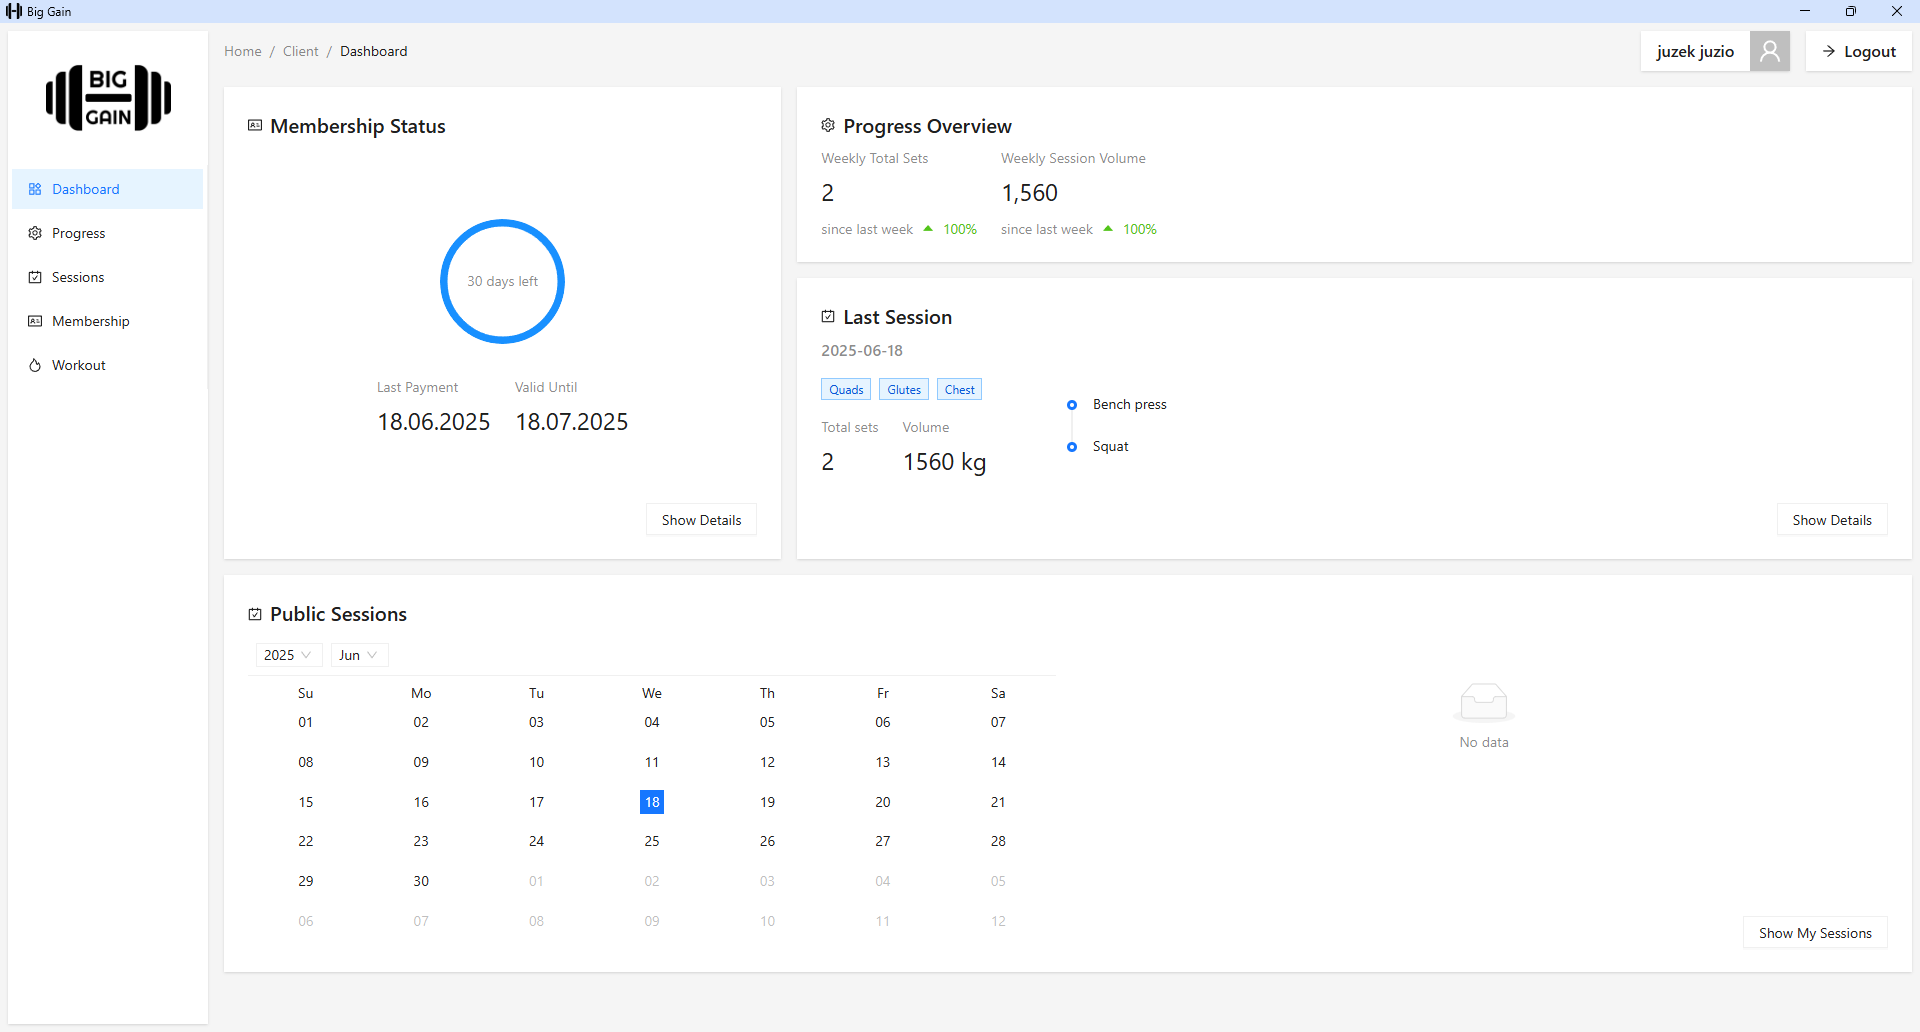
\includegraphics[width=\textwidth]{img/client.png}
  \caption{Panel klienta – przegląd statusu członkostwa, progresu oraz kalendarz sesji.}
\end{figure}

\begin{figure}[H]
  \centering
  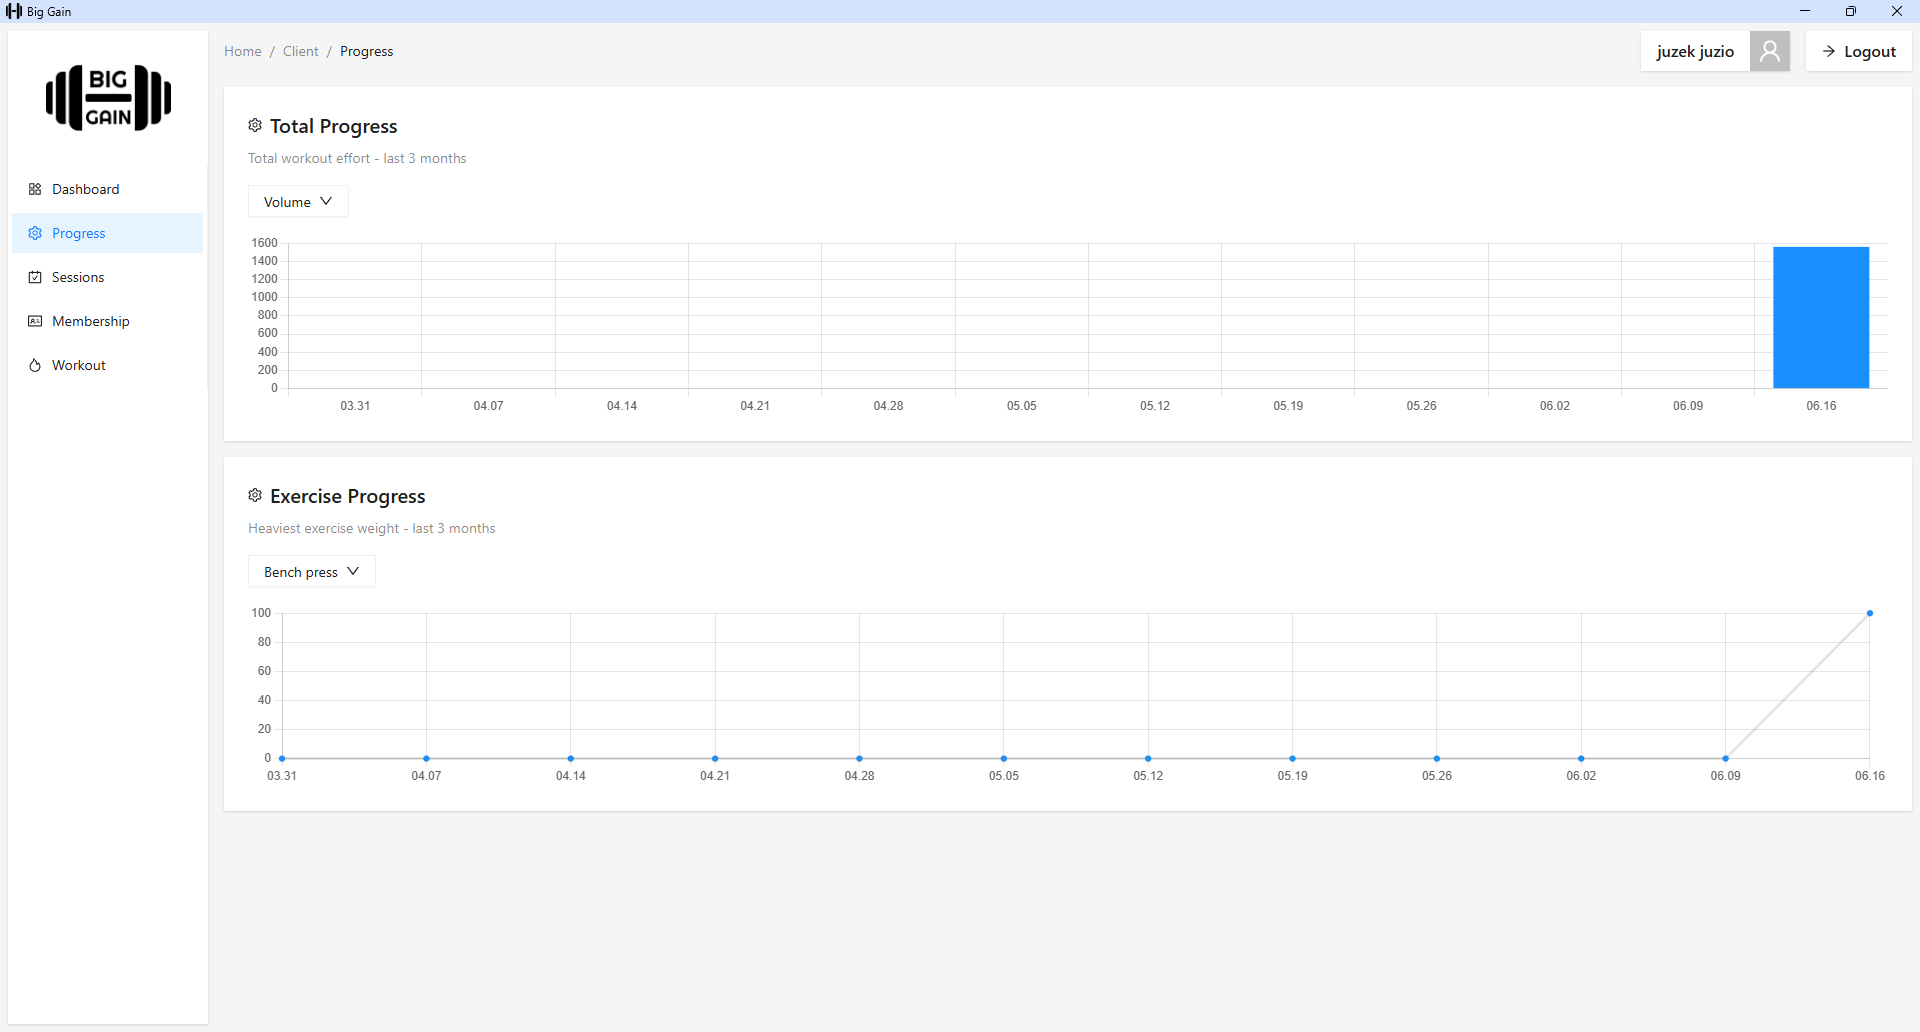
\includegraphics[width=\textwidth]{img/client_progress.png}
  \caption{Klient może śledzić swoje statystyki.}
\end{figure}

\begin{figure}[H]
  \centering
  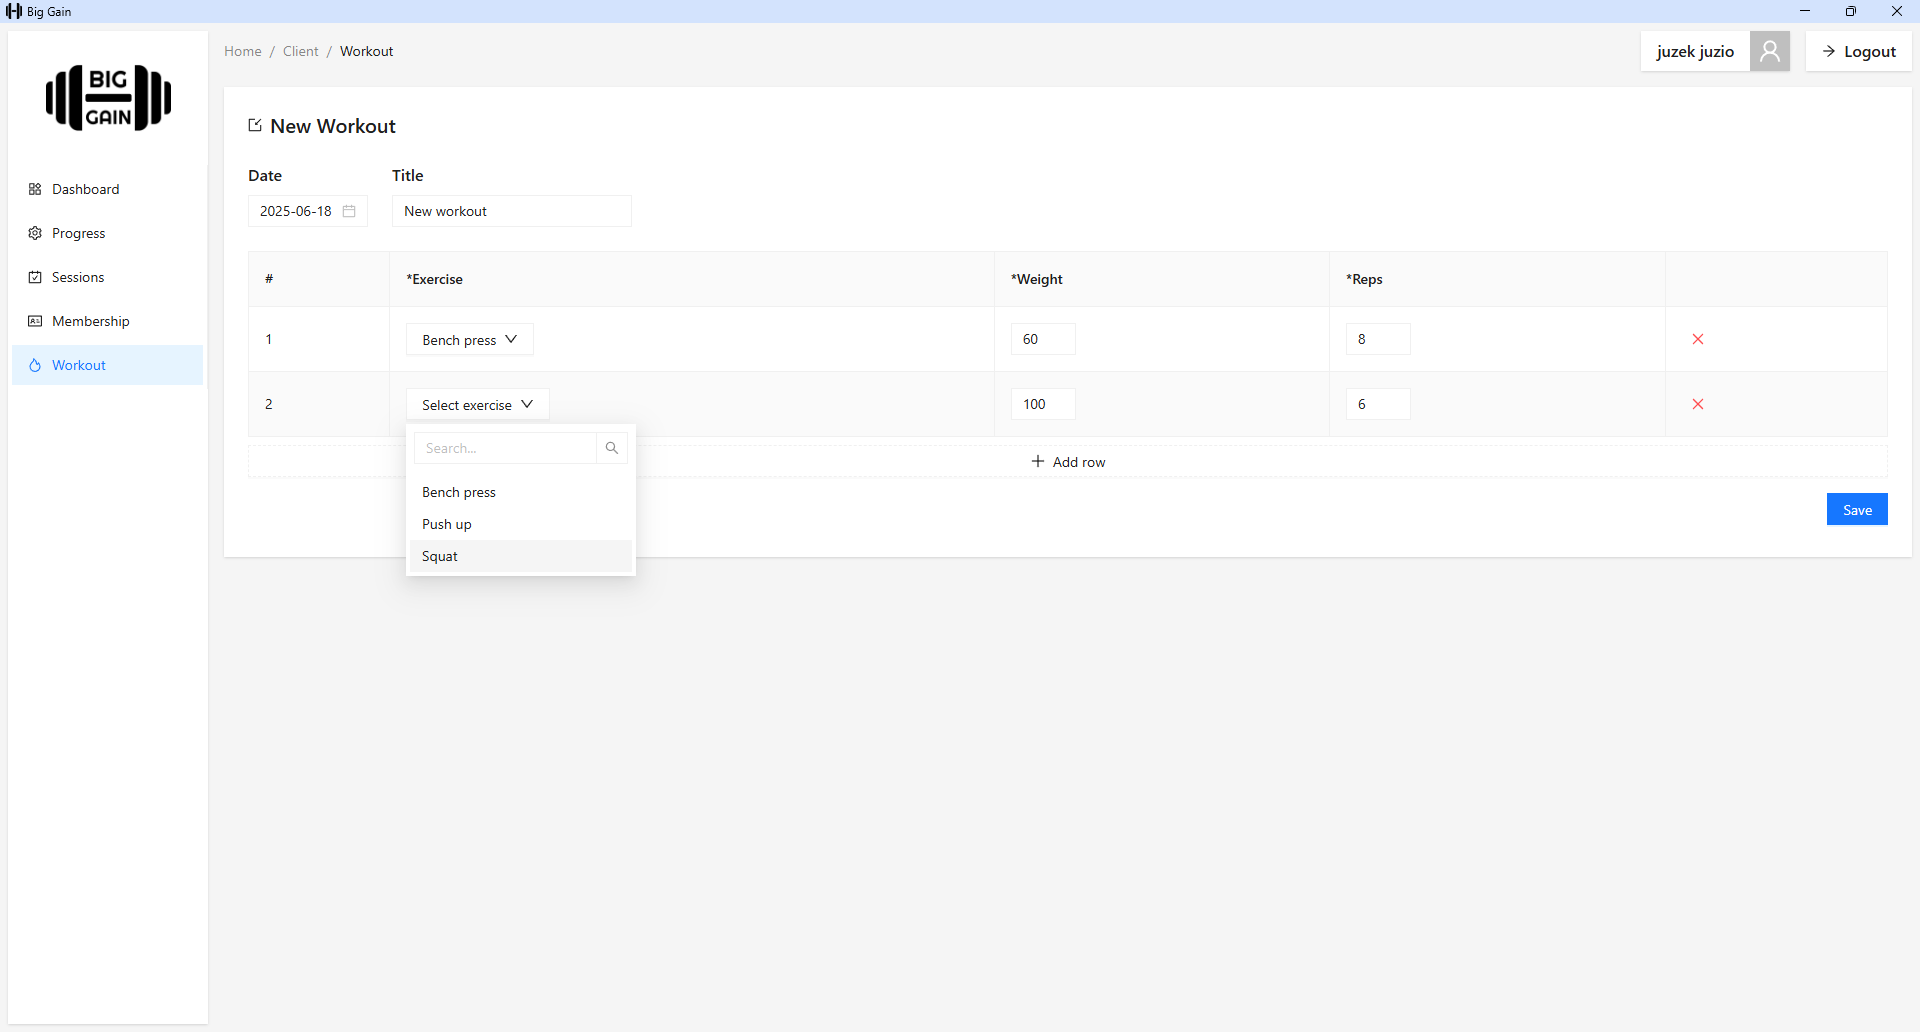
\includegraphics[width=\textwidth]{img/new_workout.png}
  \caption{Nowy trening - klient może tworzyć własne sesje.}
\end{figure}

\begin{figure}[H]
  \centering
  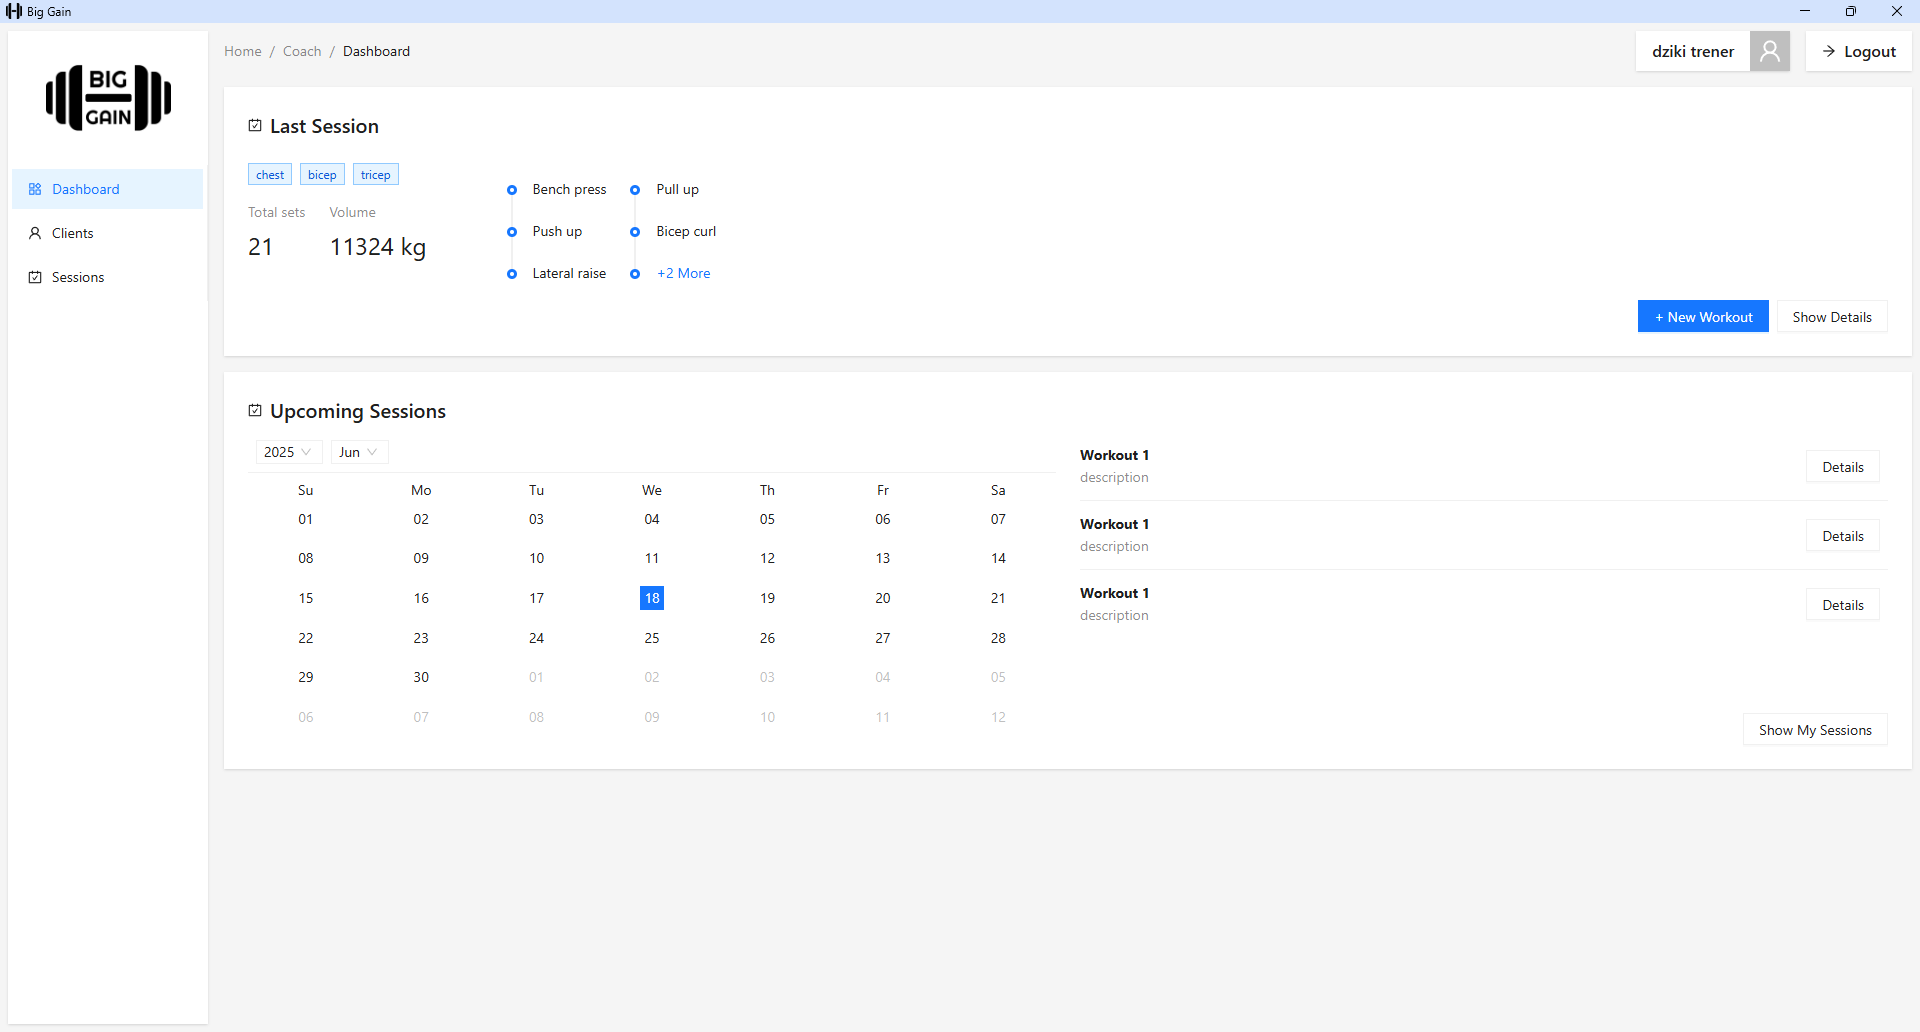
\includegraphics[width=\textwidth]{img/coach_dashboard.png}
  \caption{Panel trenera - ostatni trening, kalendarz nadchodzących sesji.}
\end{figure}

\begin{figure}[H]
  \centering
  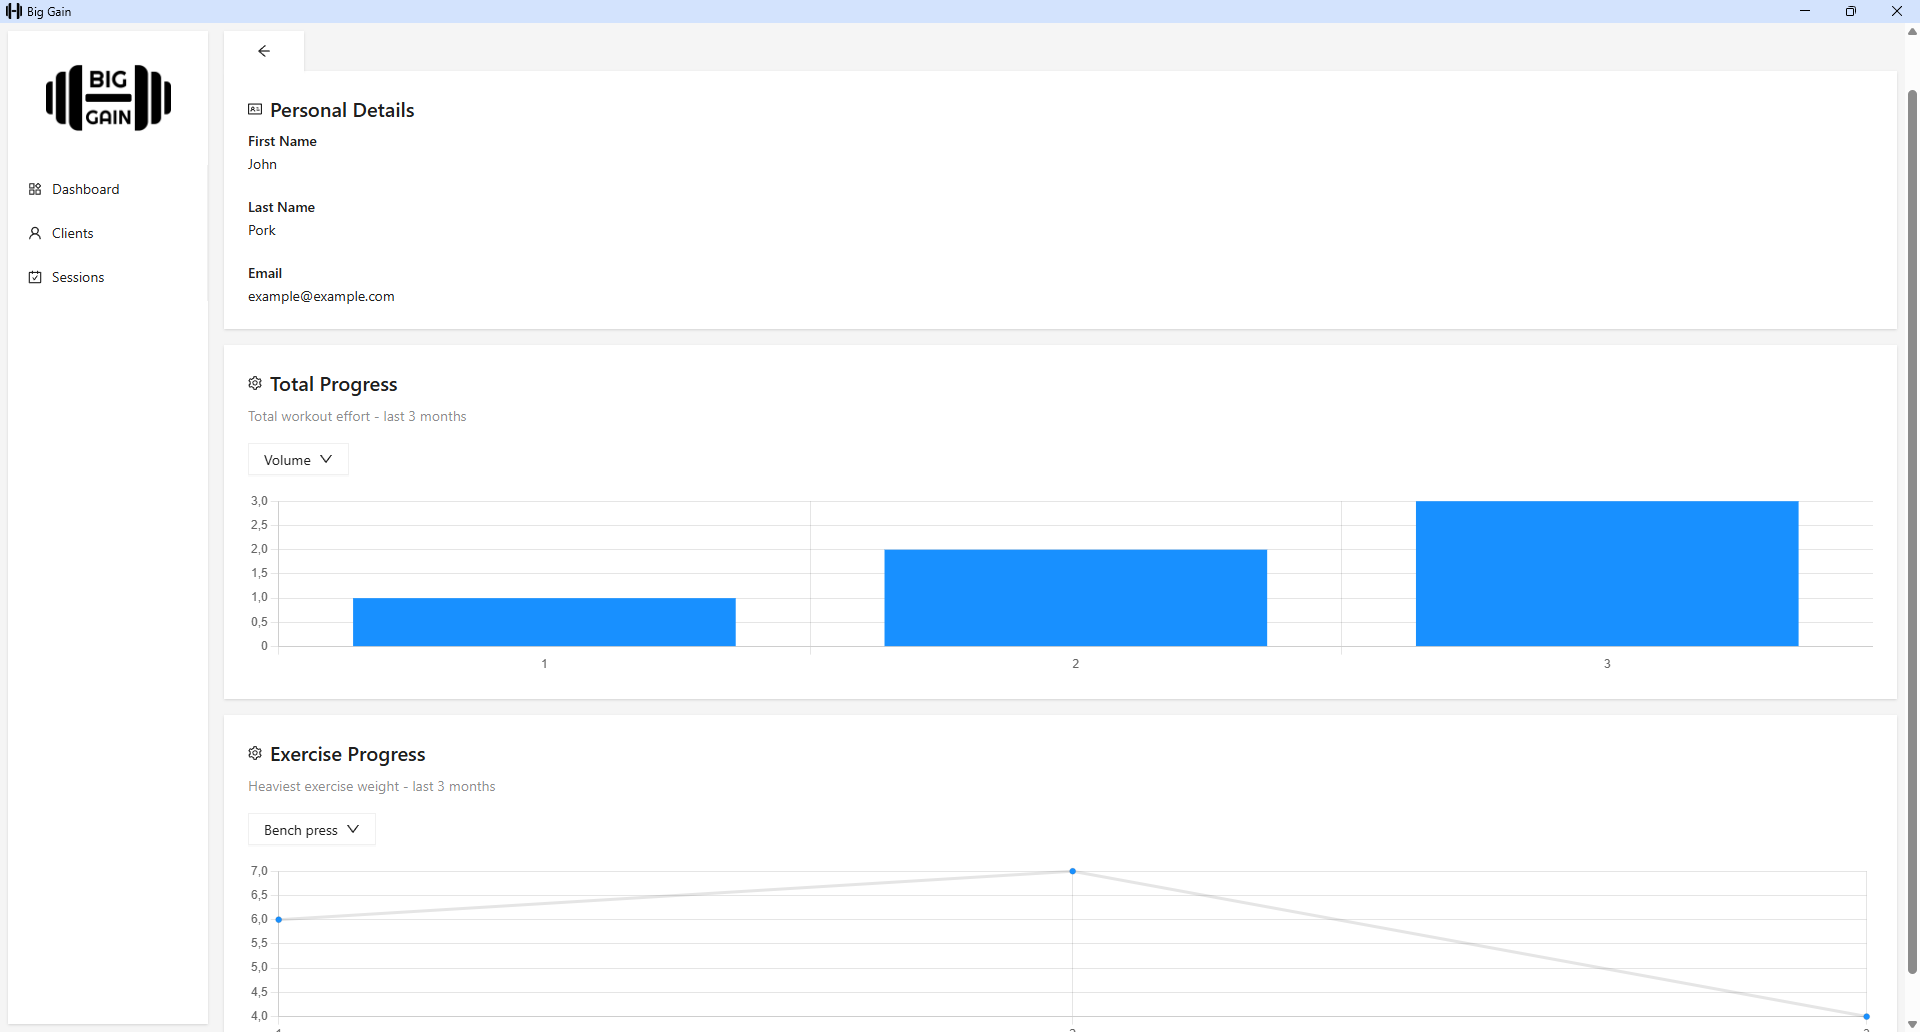
\includegraphics[width=\textwidth]{img/coach_client.png}
  \caption{Również trener może przeglądać statystyki treningowe klienta.}
\end{figure}

\begin{figure}[H]
  \centering
  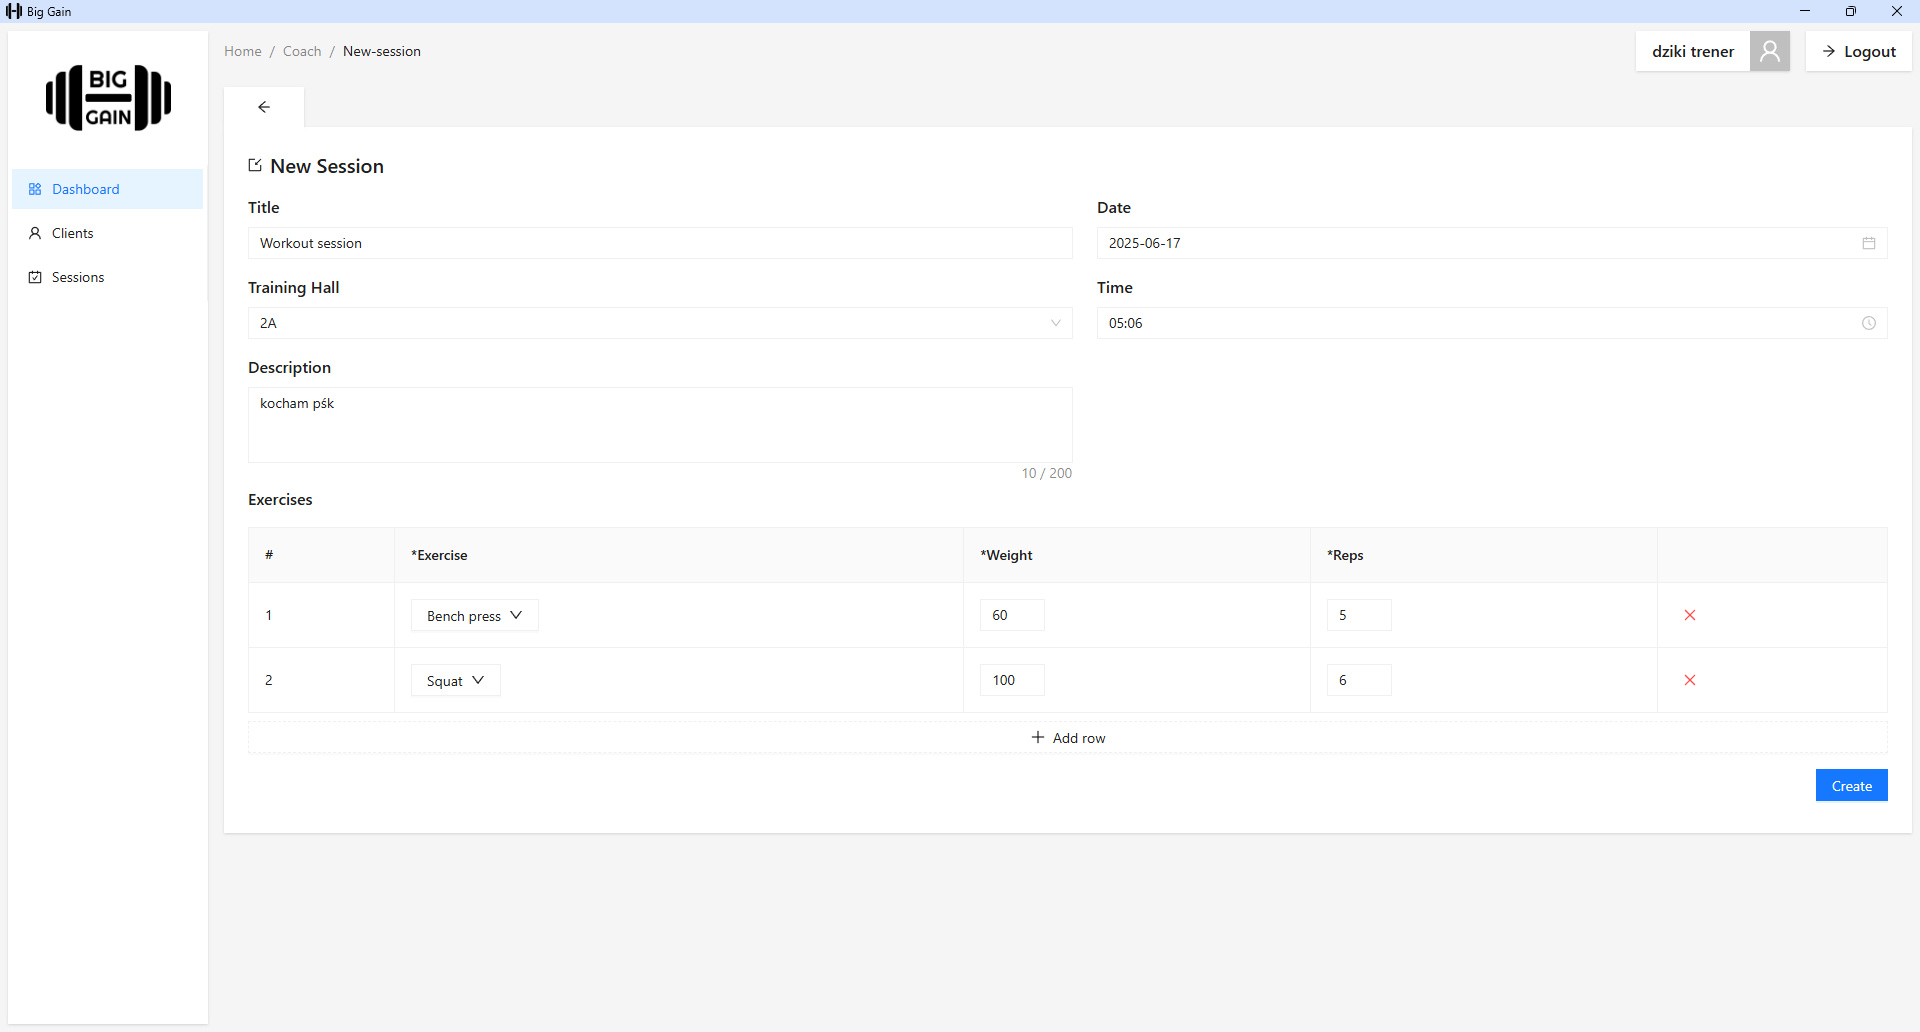
\includegraphics[width=\textwidth]{img/new_session.png}
  \caption{Tworzenie nowej sesji treningowej przez trenera.}
\end{figure}

\begin{figure}[H]
  \centering
  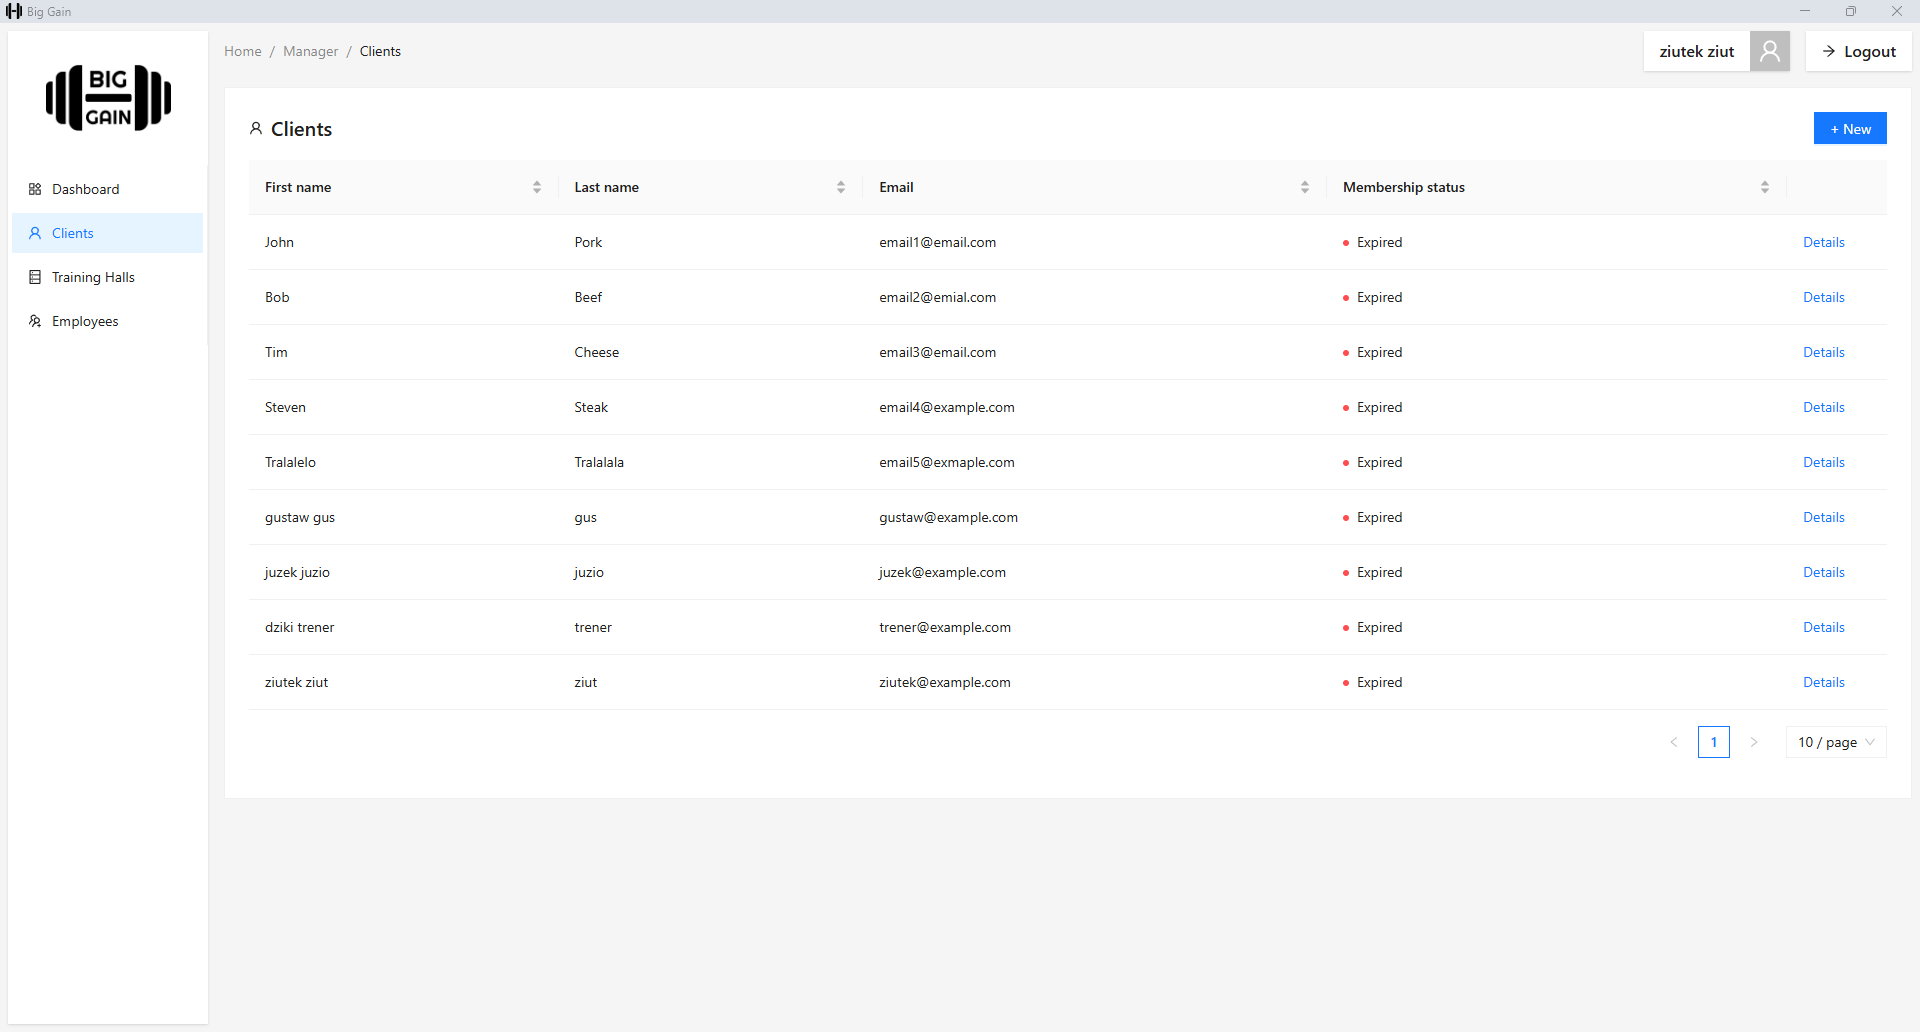
\includegraphics[width=\textwidth]{img/manager_clients.png}
  \caption{Manager jak i pracownik mają dostęp do wszystkich klientów.}
\end{figure}

\begin{figure}[H]
  \centering
  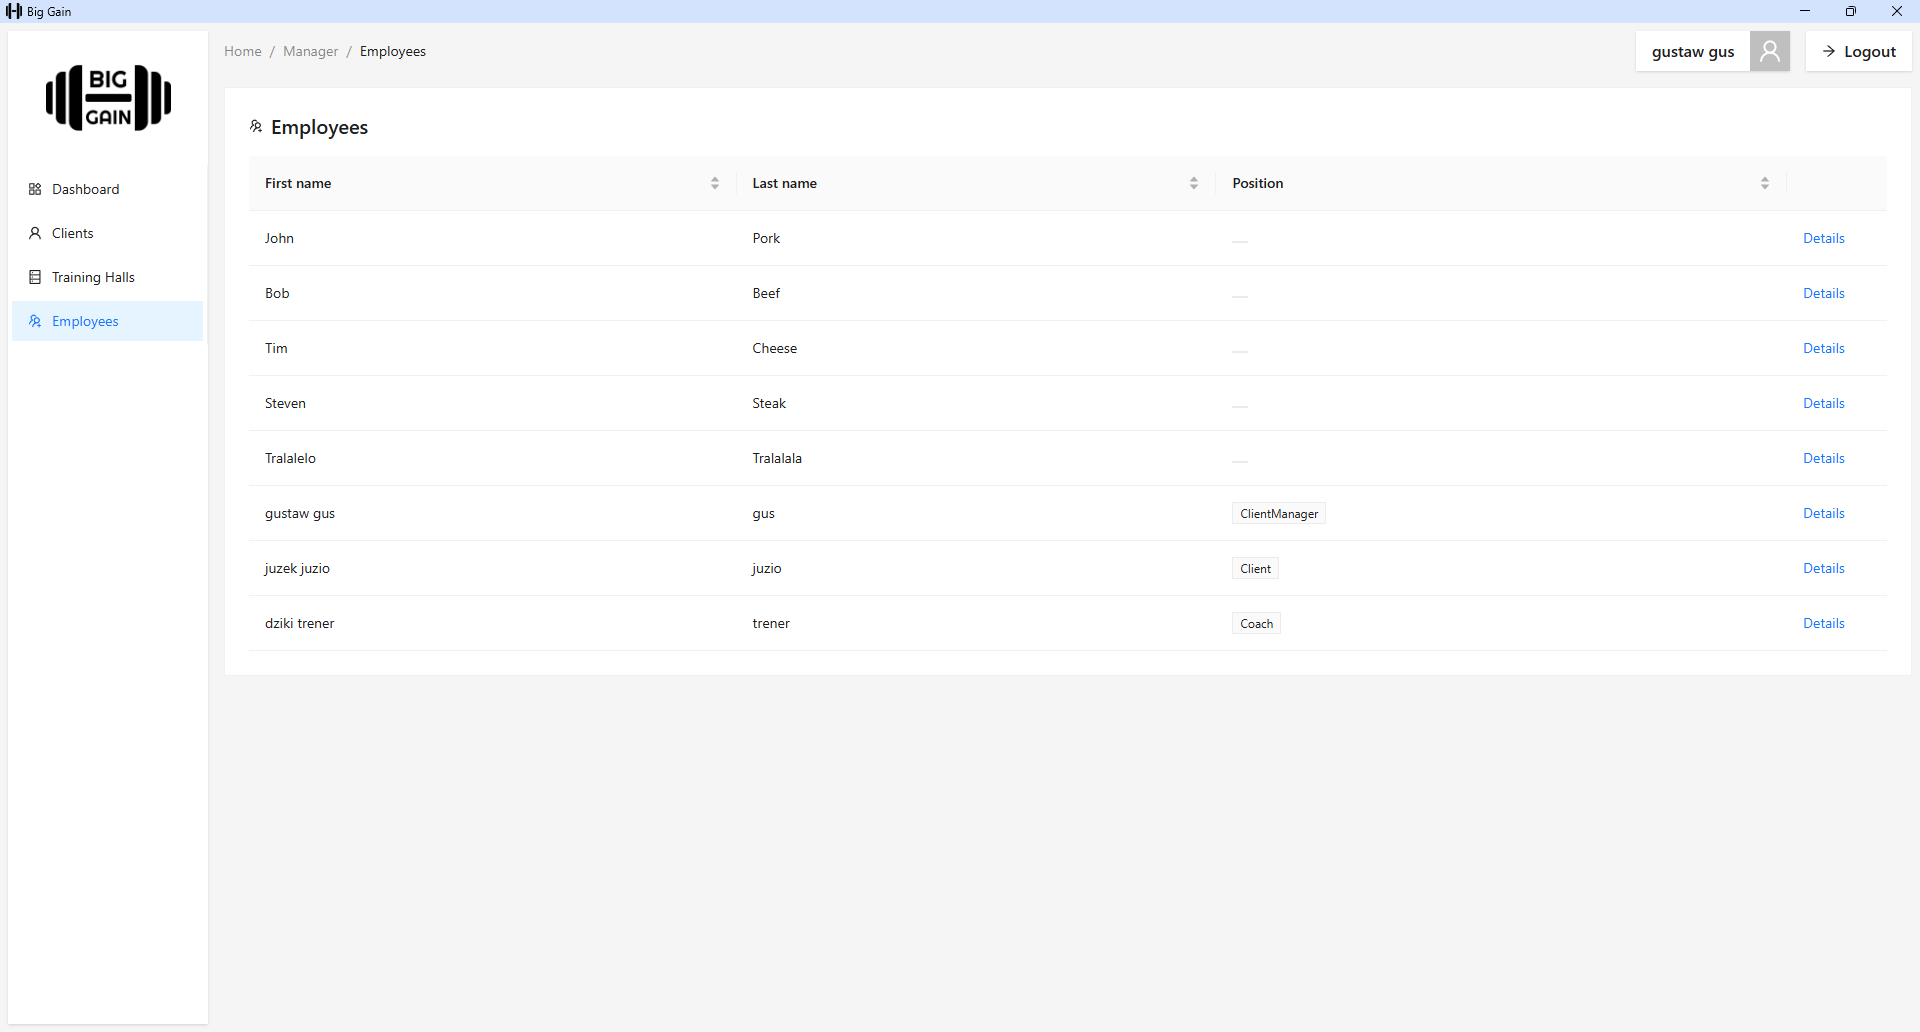
\includegraphics[width=\textwidth]{img/manager.png}
  \caption{Manager może przeglądać dane pracowników.}
\end{figure}

\begin{figure}[H]
  \centering
  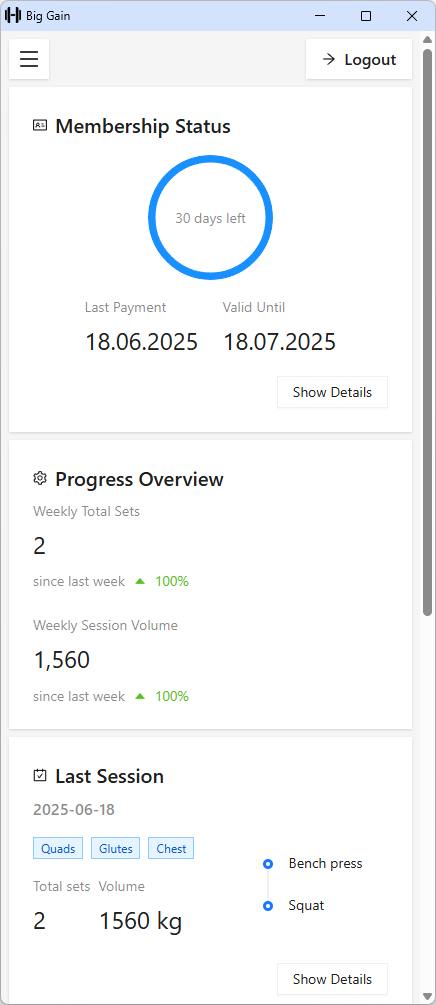
\includegraphics[width=0.35\textwidth]{img/client_dashboard_responsive.png}
  \caption{Panel użytkownika na urządzeniu mobilnym - cała aplikacja jest responsywna.}
\end{figure}


\subsection{Wybrane fragmenty kodu z kluczowymi funkcjonalnościami}

\begin{lstlisting}[caption=Przykład logiki obliczeniowej w komponencie. Funkcje służą do wyznaczania wskaźników statusu karnetu dla komponentu \textit{Progress} z \textit{Ant Design}.]
function getValidityLabel(lastPayment?: Dayjs, validUntil?: Dayjs) {
    if (!lastPayment || !validUntil) {
        return 'Expired';
    }

    const now = dayjs();
    const until = dayjs(validUntil);

    if (until.isBefore(now)) {
        return 'Expired';
    }

    const diffDays = until.diff(now, 'day');
    const diffDayjsWithToday = diffDays + 1;

    if (diffDays >= 1) {
        return `${diffDayjsWithToday} day${diffDayjsWithToday === 1 ? '' : 's'} left`;
    }

    const diffHours = until.diff(now, 'hour');
    return `${diffHours} hour${diffHours === 1 ? '' : 's'} left`;
}

function getCirclePercentage(lastPayment?: Dayjs, validUntil?: Dayjs): number {
    if (!lastPayment || !validUntil) return 0;

    const now = dayjs();

    if (now.isAfter(validUntil, 'day')) return 0;
    if (now.isBefore(lastPayment, 'day')) return 100;

    const total = validUntil.diff(lastPayment, 'days');
    const elapsed = now.diff(lastPayment, 'days');

    return Math.min(100, Math.max(0, (1 - elapsed / total) * 100));
}

// ...
const { lastPayment, validUntil } = props;
const lastPaymentDate = dayjs(lastPayment);
const validUntilDate = dayjs(validUntil);

<Progress
        type='circle'
        percent={
            lastPayment && validUntilDate
                ? getCirclePercentage(lastPaymentDate, validUntilDate)
                : 0
        }
        format={() => (
            <div className='text-font-secondary text-sm'>
                {getValidityLabel(lastPaymentDate, validUntilDate)}
            </div>
        )}
        size={125}
    />
// ...
\end{lstlisting}

\begin{lstlisting}[caption=Przykład tworzenia wykresów. Komponent generuje wykres \textit{Chart.js} na podstawie przekazanych parametrów. Możliwe jest wybranie typu wykresu oraz rozwijanej listy z kategoriami.]
export function Chart(props: ChartProps) {
    const { chartData, type, className, dropdownType } = props;

    const initialChartDataEntry = chartData?.data?.at(0);

    const [chartDataEntry, setChartDataEntry] = useState<ChartEntry | undefined>(
        initialChartDataEntry
    );

    useEffect(() => {
        setChartDataEntry(initialChartDataEntry);
    }, [initialChartDataEntry]);

    if (!chartData) {
        return <Empty />;
    }

    const menuItems = chartData.data.map(({ title }) => ({ key: title, label: title }));

    const dataExists =
        chartDataEntry &&
        chartDataEntry.timeSeries.labels.length > 0 &&
        chartDataEntry.timeSeries.values.length > 0;

    const chartComponentData = {
        labels: chartDataEntry?.timeSeries.labels,
        datasets: [
            {
                data: chartDataEntry?.timeSeries.values,
                backgroundColor: getCSSVariable('--color-primary')
            }
        ]
    };

    const handleMenuItemSelect = (item: { key: string; label: string }) => {
        const dataEntry = chartData.data.find(({ title }) => title === item.key);
        setChartDataEntry(dataEntry);
    };

    const menu =
        dropdownType === 'search' ? (
            <SearchDropdown
                placeholder={initialChartDataEntry?.title ?? 'Select'}
                menuItems={menuItems}
                onSelect={handleMenuItemSelect}
            />
        ) : (
            <Dropdown
                placeholder={initialChartDataEntry?.title ?? 'Select'}
                menuItems={menuItems}
                onSelect={handleMenuItemSelect}
            />
        );

    const chart =
        type === 'line' ? (
            <Line options={chartComponentOptions} data={chartComponentData} />
        ) : (
            <Bar options={chartComponentOptions} data={chartComponentData} />
        );

    return (
        <Flex vertical>
            <Text className='text-font-secondary mb-middle'>{chartData.description}</Text>
            {menu}
            <div className={`pt-middle min-h-50 ${className}`}>
                {dataExists ? chart : <Empty />}
            </div>
        </Flex>
    );
}
\end{lstlisting}

\begin{lstlisting}[caption=Przykład generowania tabeli. Tworzenie tabeli w każdym przypadku odbywa się za pośrednictwem komponentu \textit{Table} z \textit{Ant Design}.]
const columns: TableColumnsType<DataType> = [
    {
        title: 'First name',
        dataIndex: 'firstName',
        key: 'firstName',
        fixed: 'left',
        sorter: (a, b) => a.firstName.localeCompare(b.firstName)
    },
    {
        title: 'Last name',
        dataIndex: 'lastName',
        key: 'lastName',
        sorter: (a, b) => a.lastName.localeCompare(b.lastName)
    },
    {
        title: 'Position',
        dataIndex: 'position',
        key: 'position',
        sorter: (a, b) => a.position.localeCompare(b.position),
        render: (position: string) => <Tag>{position}</Tag>
    },

    {
        key: 'detailsHref',
        dataIndex: 'detailsHref',
        fixed: 'right',
        width: 100,
        render: (href: string) => <Link to={href}>Details</Link>
    }
];

export function EmployeesTableCard({ employees = [], newEmployeeHref }: EmployeesTableCardProps) {
    return (
        <Card className='w-full'>
            <Flex vertical className='gap-layout'>
                <Flex justify='space-between'>
                    <CardTitle title='Employees' icon='employees' />
                    {newEmployeeHref && (
                        <ActionButton primary href={newEmployeeHref}>
                            + New
                        </ActionButton>
                    )}
                </Flex>
                <Table<DataType>
                    pagination={false}
                    columns={columns}
                    dataSource={employees.map((e, i) => ({ key: i, ...e }))}
                    scroll={{ x: 'max-content' }}
                />
            </Flex>
        </Card>
    );
}
\end{lstlisting}

\begin{lstlisting}[caption=Przykład obsługi formularza. Wykorzystywany jest \textit{hook useForm} z \textit{Ant Design} który pozwala na łatwą walidację i przesyłanie wartości z formularza.]
export function HallCreationCard({ hallTypes = [], onCreate = () => {} }: HallCreationCardProps) {
    const [form] = Form.useForm();

    return (
        <Card>
            <CardTitle title='Create Hall' icon='training-halls' />
            <Form
                form={form}
                layout='vertical'
                onFinish={onCreate}
                requiredMark={label => <span>{label}</span>}
                className='pt-small'
            >
                <Flex className='gap-layout'>
                    <Flex vertical className='w-full'>
                        <Form.Item
                            label='Hall Number'
                            name='hallNumber'
                            rules={[{ required: true, message: '' }]}
                        >
                            <Input placeholder='Enter hall number' />
                        </Form.Item>

                        <Form.Item
                            label='Type'
                            name='hallType'
                            rules={[{ required: true, message: '' }]}
                        >
                            <Select placeholder='Select hall type'>
                                {hallTypes.filter(Boolean).map(type => (
                                    <Select.Option key={type.name} value={type.uuid}>
                                        {type.name}
                                    </Select.Option>
                                ))}
                            </Select>
                        </Form.Item>
                    </Flex>

                    <Flex className='w-full' vertical>
                        <Form.Item
                            label='Description'
                            name='hallDescription'
                            rules={[{ required: true, message: '' }]}
                        >
                            <TextArea rows={5} placeholder='Enter description' allowClear />
                        </Form.Item>
                    </Flex>
                </Flex>

                <Flex justify='end'>
                    <Button type='primary' htmlType='submit'>
                        Create
                    </Button>
                </Flex>
            </Form>
        </Card>
    );
}
\end{lstlisting}

\begin{lstlisting}[caption=Przykład globalnego stanu aplikacji. \textit{UserProvider} dostarcza innym komponentom kontekst użytkownika pobrany z serwisu \textit{Keycloak}.]
export function UserProvider({ children }: { children: JSX.Element }) {
    const [userDetails, setUserDetails] = useState<UserDetails>();

    const updateUser = (updates: Partial<UserDetails>) => {
        setUserDetails(prev => (prev ? { ...prev, ...updates } : prev));
    };

    useEffect(() => {
        async function initUser() {
            const initialized = await keycloak.init({ onLoad: 'login-required' });
            if (!initialized) return;

            initializeAxios(keycloak);

            const userProfile = await keycloak.loadUserProfile();
            const userRoles = keycloak.tokenParsed?.['roles'] as UserRole[];
            console.log(keycloak.tokenParsed);
            const significantRole = userRoles
                .sort((a: UserRole, b: UserRole) => rolesPriority[b] - rolesPriority[a])
                .at(0);

            const whoAmIData = await whoAmI()
                .then(data => data?.data)
                .catch(() => {
                    console.error('failed to fetch user data. Is backend API online ?');
                    return undefined;
                });

            const userDetails: UserDetails = {
                firstName: userProfile.firstName as string,
                lastName: userProfile.lastName as string,
                email: userProfile.email as string,
                role: significantRole ?? 'client',
                id: whoAmIData?.uuid,
                hasValidMembership: dayjs().isBefore(dayjs(whoAmIData?.membership?.validUntil))
            };

            setUserDetails(userDetails);
        }

        if (import.meta.env.VITE_AUTH_ENABLED === 'true') {
            initUser();
        }
    }, []);

    return (
        <UserContext.Provider value={{ user: userDetails, updateUser }}>
            {children}
        </UserContext.Provider>
    );
}
\end{lstlisting}

\begin{lstlisting}[caption=Przykład niestandardowego \textit{hooka}. Służy do obserwacji szerokości elementu i jest wykorzsytany przy obsłudze responsywności.]
export function useHTMLElementResizeObserver<T extends HTMLElement = HTMLDivElement>() {
    const ref = useRef<T>(null);
    const [width, setWidth] = useState(0);

    useEffect(() => {
        if (!ref.current) return;
        const observer = new ResizeObserver(entries => {
            for (const entry of entries) {
                const { width } = entry.contentRect;
                setWidth(width);
            }
        });

        observer.observe(ref.current);
        return () => observer.disconnect();
    }, []);

    return [ref, Math.floor(width)];
}
\end{lstlisting}

\begin{lstlisting}[caption=Przykład komponentu pobierającego dane z zewnętrznego API. Wykorzystywane są funkcje generowane przez \textit{Orval} co eliminuje konieczność ręcznego korzystania z biblioteki \textit{axios}.]
export function MembershipStatusCardWithData({ horizontal, showDetails }: MembershipStatusCardWithDataProps) {
    const { user } = useUser();
    const [membership, setMembership] = useState<Membership>();

    useEffect(() => {
        async function getMembershipStatus() {
            if (!user?.id) return;
            const userMembership = (await getUser(user.id)).data.membership;
            setMembership(userMembership);
        }

        getMembershipStatus();
    }, [user?.id]);

    return (
        <MembershipStatusCard
            detailsHref={showDetails ? `/${user?.role}/membership` : undefined}
            lastPayment={membership?.validFrom}
            validUntil={membership?.validUntil}
            horizontal={horizontal}
        />
    );
}
\end{lstlisting}

\begin{lstlisting}[caption=Komponent realizujący \textit{routing} w aplikacji. Definiuje ścieżki i komponenty generujące poszczególne ekrany.]
export function Router() {
    return (
        <BrowserRouter>
            <AuthGuard>
                <Routes>
                    <Route path='renew-membership' element={<ClientRenewMembershipPage />} />
                    <Route
                        path={rolesConfig['client'].routePrefix}
                        element={<AuthenticatedLayout renderChat={false} role='client' />}
                    >
                        <Route path='dashboard' element={<ClientDashboardPage />} />
                        <Route path='progress' element={<ClientProgressPage />} />
                        <Route path='sessions' element={<SessionsPage />} />
                        <Route path='membership' element={<ClientMembershipPage />} />
                        <Route path='workout' element={<ClientWorkoutPage />} />
                        <Route path='workout/:id' element={<WorkoutDetailsPage />} />
                    </Route>

                    <Route
                        path={rolesConfig['employee'].routePrefix}
                        element={<AuthenticatedLayout renderChat={false} role='employee' />}
                    >
                        <Route path='dashboard' element={<EmployeeDashboardPage />} />
                        <Route path='clients' element={<ClientsPage />} />
                        <Route path='training-halls' element={<HallsPage />} />
                        <Route path='create-membership' element={<MembershipCreationPage />} />
                        <Route path='clients/:id' element={<ClientDetailsPage />} />
                        <Route path='training-halls/:id' element={<EmployeeHallDetailsPage />} />
                    </Route>

                    <Route
                        path={rolesConfig['coach'].routePrefix}
                        element={<AuthenticatedLayout renderChat={false} role='coach' />}
                    >
                        <Route path='dashboard' element={<CoachDashboardPage />} />
                        <Route path='clients' element={<ClientsPage />} />
                        <Route path='sessions' element={<SessionsPage />} />
                        <Route path='workout/:id' element={<WorkoutDetailsPage />} />
                        <Route path='clients/details/:id' element={<CoachClientDetailsPage />} />
                        <Route path='new-session' element={<CoachNewSessionPage />} />
                    </Route>

                    <Route
                        path={rolesConfig['manager'].routePrefix}
                        element={<AuthenticatedLayout renderChat={false} role='manager' />}
                    >
                        <Route path='dashboard' element={<ManagerDashboardPage />} />
                        <Route path='create-membership' element={<MembershipCreationPage />} />
                        <Route path='clients' element={<ClientsPage />} />
                        <Route path='clients/:id' element={<ClientDetailsPage />} />
                        <Route path='employees' element={<ManagerEmployeesPage />} />
                        <Route path='create-employee' element={<ManagerEmployeeCreationPage />} />
                        <Route path='employees/:id' element={<ManagerEmployeeDetailsPage />} />
                        <Route path='client-details' element={<ClientDetailsPage />} />
                        <Route path='training-halls' element={<HallsPage />} />
                        <Route path='training-halls/details/:id' element={<div></div>} />
                        <Route path='create-hall' element={<ManagerHallCreationPage />} />
                    </Route>
                </Routes>
            </AuthGuard>
        </BrowserRouter>
    );
}
\end{lstlisting}

\newpage

\begin{lstlisting}[caption=Komponent chroniący podstrony - zapewnia przekierowania i wymusza logowanie użytkownika.]
export function AuthGuard({ children }: AuthGuardProps) {
    const { user } = useUser();
    const location = useLocation();
    const [loading, setLoading] = useState(false);

    useEffect(() => {
        setLoading(user === undefined);
    }, [user]);

    const isPublicPath = PUBLIC_PATHS.some(path => location.pathname.startsWith(path));

    if (import.meta.env.VITE_AUTH_ENABLED === 'false' || isPublicPath) {
        return children;
    }

    if (loading || !user) {
        return <Loader />;
    }

    const { routePrefix, defaultRoute } = rolesConfig[user?.role];
    const isPathAllowed = location.pathname.startsWith(routePrefix);

    if (!isPathAllowed) {
        return <Navigate to={routePrefix + defaultRoute} replace />;
    } else if (isPathAllowed && user.role === 'client' && !user.hasValidMembership) {
        return <Navigate to='/renew-membership' />;
    } else {
        return children;
    }
}
\end{lstlisting}

\end{document}